\documentclass[conference]{IEEEtran}
\usepackage{xeCJK}
\usepackage{zhnumber}
\usepackage{indentfirst}
\usepackage{amsmath,amssymb,amsfonts}
\usepackage{graphicx}
\usepackage{algorithm}
\usepackage{algorithmic}
\usepackage{booktabs}
\usepackage{multirow}
\usepackage{cite}
\usepackage{color}
\usepackage{listings}
\usepackage{url}
\usepackage{subfigure}
\usepackage{placeins} % 引入 placeins 套件以使用 \FloatBarrier

% 保持原有字型設定
\setCJKmainfont{SimSun}
\setCJKsansfont{SimHei}
\setCJKmonofont{SimSun}

\lstset{
    basicstyle=\footnotesize\ttfamily,
    breaklines=true,
    keywordstyle=\color{blue},
    commentstyle=\color{olive},
    stringstyle=\color{red},
    frame=single,
    numbers=left,
    numbersep=5pt,
    numberstyle=\tiny
}

\begin{document}

\title{房間佈置優化:模擬退火與精確解法的比較研究}

\author{
    \IEEEauthorblockN{李則霖}
    \IEEEauthorblockA{軟創三乙 511172176\\
    資訊工程學系\\
    輔仁大學}
}

\maketitle

\begin{abstract}
在有限室內空間中,自動化優化房間佈置能協助設計師快速找到高品質佈局方案。本研究比較模擬退火(Simulated Annealing, SA)與精確解法(Exact Solver)兩種方法在房間佈置優化問題中的表現。我們選取四種不同規模的房間案例(3×3m、5×4m、2.5×2m、6×5m)進行實驗,分析其運行時間與能量(品質)表現。結果顯示:精確解法在小規模問題中能快速求得最優解,SA亦可達同品質解但耗時較長;在中大型問題中,精確解法無法求解(N/A),SA則雖耗時但可取得可行解。此外,我們提供整合的能量與時間比較圖,以更清楚呈現兩方法的優缺點。

\textbf{關鍵詞}---模擬退火、精確解法、房間佈置、空間優化、自動化設計
\end{abstract}

\section{引言}
在室內設計中,家具的合理佈置攸關空間利用率與舒適度。傳統設計仰賴經驗,難以確保全域最優性。透過將問題轉化為組合優化並套用先進演算法,我們可在可控制時間內找到高品質解。

本研究比較模擬退火(SA)與精確解法(Exact Solver)於房間佈置優化問題之適用性。SA可在大規模問題中尋得近似解\cite{b1},精確解法在小問題可保證最優解但不適用於中大型問題\cite{b2}。

\section{研究背景與方法}
\subsection{問題定義與能量機制}
給定房間 \( R(w,h) \) 與家具集合 \( F \)。每家具具有固定尺寸與可擺放位置、旋轉方向(0°或90°)。為衡量佈局品質,定義能量函數:

\begin{align}
\min E &= \sum_{i=1}^{n}\sum_{j=i+1}^{n} O_{ij} + \sum_{i=1}^{n} B_i, \label{eq:energy} \\
O_{ij} &= \max\left(0, \min(x_i + w_i, x_j + w_j) - \max(x_i, x_j)\right) \nonumber \\
&\quad \times \max\left(0, \min(y_i + h_i, y_j + h_j) - \max(y_i, y_j)\right), \label{eq:overlap} \\
B_i &= \max\left(0, x_i + w_i - R_w\right) + \max\left(0, y_i + h_i - R_h\right). \label{eq:boundary}
\end{align}

其中:
\begin{itemize}
    \item \( O_{ij} \) 為家具 \( i \) 與家具 \( j \) 之間的重疊面積。當 \( O_{ij} > 0 \) 時,表示兩家具重疊。
    \item \( B_i \) 為家具 \( i \) 的越界懲罰,確保家具不超出房間範圍。能量越低,佈局品質越佳。
\end{itemize}

\subsection{模擬退火 (SA) 虛擬碼}
{\small
\begin{algorithm}[!htbp]
\caption{Simulated Annealing (SA) Pseudocode}
\begin{algorithmic}[1]
\STATE Generate initial solution \( S \)
\STATE \( T = T_0 \) \textbf{(initial temperature)}
\WHILE{\( T > T_{\text{min}} \)}
    \FOR{\( k=1 \) to \( L \)}
        \STATE \( S' = \text{GenerateNeighbor}(S) \)
        \STATE \( \Delta E = E(S') - E(S) \)
        \IF{\( \Delta E < 0 \) \textbf{or} \( e^{-\frac{\Delta E}{T}} > \text{rand}(0,1) \)}
            \STATE \( S \leftarrow S' \)
        \ENDIF
    \ENDFOR
    \STATE \( T \leftarrow \alpha \cdot T \)
\ENDWHILE
\RETURN \( S \)
\end{algorithmic}
\end{algorithm}
}

SA 以高溫階段允許較差解被接受以逃離局部極值,隨降溫逐漸收斂至優解。

\subsection{模擬退火(SA)數學描述}
模擬退火是一種啟發式搜尋算法,用於在大規模搜索空間中找到近似全域最優解。

**接受新狀態的概率**:
\[
P = 
\begin{cases} 
1 & \Delta E \leq 0, \\
e^{-\frac{\Delta E}{T}} & \Delta E > 0.
\end{cases}
\]
其中:
\begin{itemize}
    \item \( \Delta E = E_{\text{new}} - E_{\text{current}} \) 是新佈局的能量變化。
    \item \( T \) 是當前溫度,隨迭代逐漸降低。
\end{itemize}

**降溫公式**:
\[
T_{\text{new}} = \alpha \cdot T_{\text{current}}
\]
其中:
\begin{itemize}
    \item \( \alpha \) 是降溫速率,程式中設置為 \( 0.85 \)。
    \item \( T_{\text{initial}} \) 是初始溫度,程式中設置為 \( 5000 \)。
\end{itemize}

\subsection{精確解法 (Exact Solver) 虛擬碼}
\begin{algorithm}[!htbp]
\caption{Exact Solver (Branch and Bound) Pseudocode}
\begin{algorithmic}[1]
\STATE Initialize search tree node (empty layout), \( BestE = \infty \)
\WHILE{Queue not empty}
    \STATE Node = ExtractMin(Queue)
    \IF{Node lower bound \( > BestE \)}
        \STATE Prune this node
    \ELSE
        \STATE Expand node: place next furniture
        \FOR{each feasible placement}
            \STATE Calculate \( E \) or lower bound
            \IF{All furniture placed}
                \IF{\( E < BestE \)}
                    \STATE \( BestE = E \), update solution
                \ENDIF
            \ELSE
                \STATE Insert child node
            \ENDIF
        \ENDFOR
    \ENDIF
\ENDWHILE
\RETURN BestSolution
\end{algorithmic}
\end{algorithm}

精確解法能對小問題快速找到最優解,但在中大型問題中計算爆炸性增長,以致無解(N/A),其完整虛擬碼放置於文後頁。

\subsection{精確解法(Exact Solver)數學描述}
暴力搜尋是一種枚舉所有可能佈局的算法,用於尋找全域最優解。

\[
S = \prod_{i=1}^{N} P_i
\]

其中:
\begin{itemize}
    \item \( N \) 是家具的總數。
    \item \( P_i \) 是家具 \( i \) 的所有可能位置和旋轉的排列組合數。
\end{itemize}

描述:
\begin{itemize}
    \item 每個家具的排列數由步進長度(如 \( 0.25 \) m)和房間尺寸確定。
    \item 通過遍歷 \( S \) 找到能量最小的佈局,當 \( E = 0 \) 時,即為最優解。
\end{itemize}

\FloatBarrier % 確保所有浮動物件在此之前被放置

\section{實驗設計}
本研究測試四案例:
\begin{itemize}
    \item \textbf{CASE1:} 3×3m(小規模)
    \item \textbf{CASE2:} 5×4m(中規模)
    \item \textbf{CASE3:} 2.5×2m(小規模)
    \item \textbf{CASE4:} 6×5m(大規模)
\end{itemize}

比較 SA 與精確解法之最終能量與時間。

\section{結果與分析}
以下依案例展示最優解佈局圖(精確解法與 SA 各一張,部分案例僅有 SA 圖),再呈現整體能量與時間比較,最後以表格彙整。

\subsection{CASE1 (3×3m)}
小規模,精確解法可瞬間達能量 0,SA 亦能達 0 但較久。

\begin{figure}[!htbp]
    \centering
    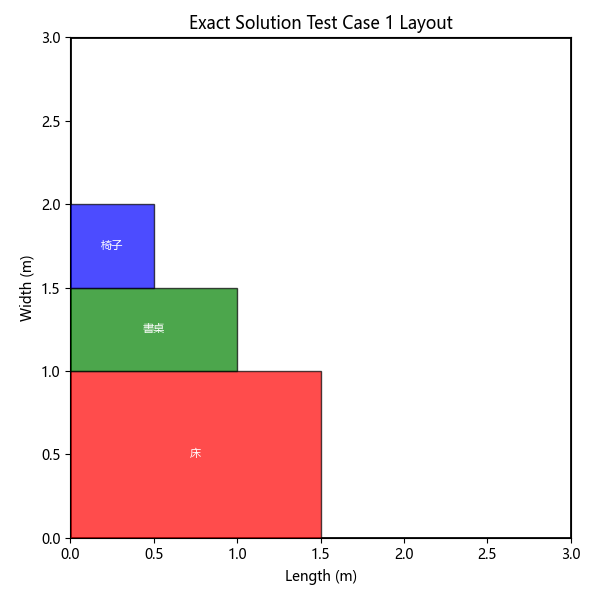
\includegraphics[width=\columnwidth]{exact_layout_test_case_1.png} 
    \caption{CASE1 精確解法最優佈局示意圖}
    \label{fig:case1_exact_solver} % 添加標籤以便在正文中引用
\end{figure}

\begin{figure}[!htbp]
    \centering
    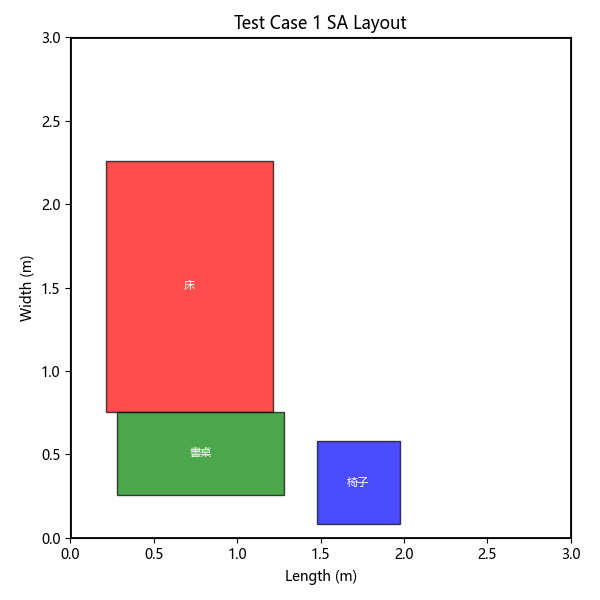
\includegraphics[width=\columnwidth]{sa_layout_test_case_1.png} 
    \caption{CASE1 SA最優佈局示意圖}
    \label{fig:case1_exact_solver} % 添加標籤以便在正文中引用
\end{figure}

\FloatBarrier % 確保 CASE1 的圖片被放置

\subsection{CASE2 (5×4m)}
中規模,精確解法無解(inf),SA 約 8.7276 秒取得能量 0 解。

\begin{figure}[!htbp]
    \centering
    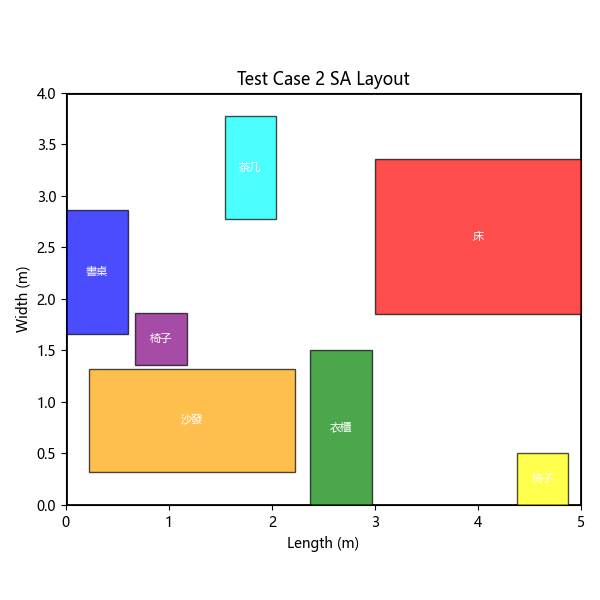
\includegraphics[width=\columnwidth]{sa_layout_test_case_2.png} 
    \caption{CASE2 SA最優佈局示意圖}
    \label{fig:case1_exact_solver} % 添加標籤以便在正文中引用
\end{figure}

\FloatBarrier % 確保 CASE2 的圖片被放置

\subsection{CASE3 (2.5×2m)}
小規模類似 CASE1,精確解法快速 0 能量,SA 亦可但耗時較長。

\begin{figure}[!htbp]
    \centering
    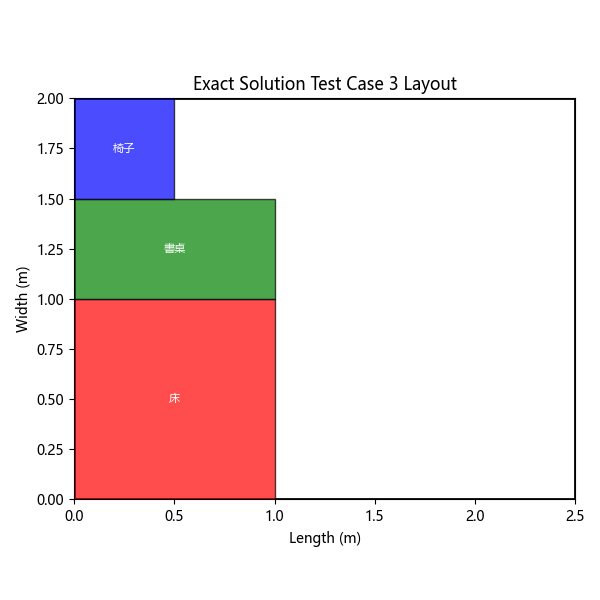
\includegraphics[width=\columnwidth]{exact_layout_test_case_3.png} 
    \caption{CASE3 精確解法最優佈局示意圖}
    \label{fig:case1_exact_solver} % 添加標籤以便在正文中引用
\end{figure}

\begin{figure}[!htbp]
    \centering
    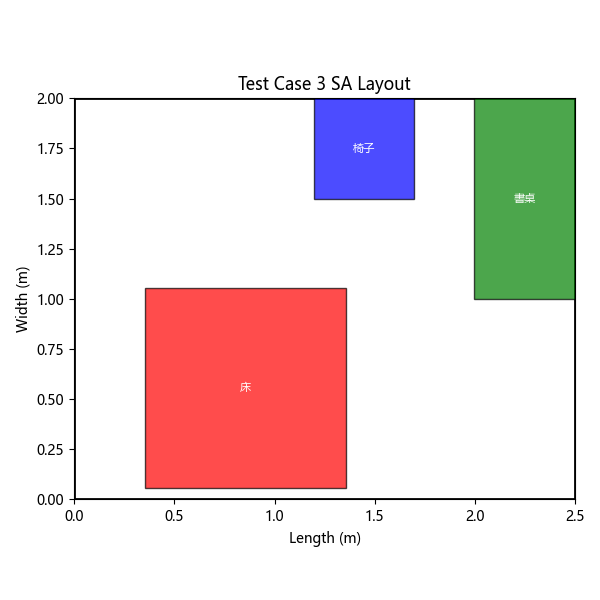
\includegraphics[width=\columnwidth]{sa_layout_test_case_3.png} 
    \caption{CASE3 SA最優佈局示意圖}
    \label{fig:case1_exact_solver} % 添加標籤以便在正文中引用
\end{figure}

\FloatBarrier % 確保 CASE3 的圖片被放置

\subsection{CASE4 (6×5m)}
大規模,精確解法無法求解(N/A),SA 約 16.3204 秒取得能量 0.39解。

\begin{figure}[!htbp]
    \centering
    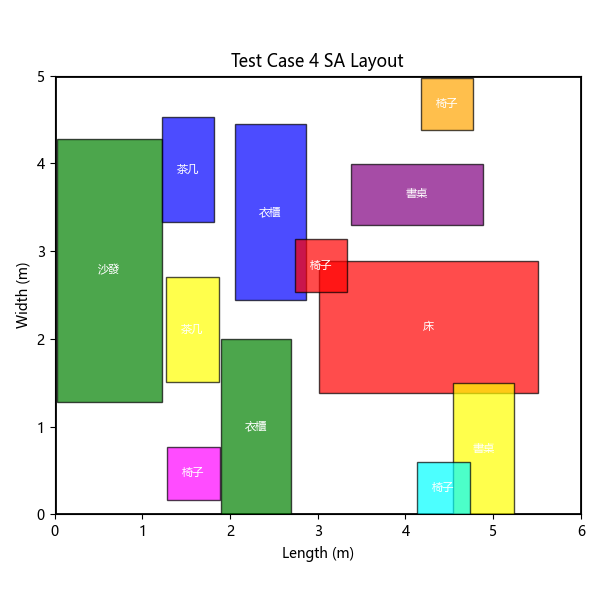
\includegraphics[width=\columnwidth]{sa_layout_test_case_4.png} 
    \caption{CASE4 SA最優佈局示意圖}
    \label{fig:case1_exact_solver} % 添加標籤以便在正文中引用
\end{figure}

\FloatBarrier % 確保 CASE4 的圖片被放置

\subsection{整體能量比較}
以下為 SA 與精確解法的能量比較圖:

\begin{figure}[!htbp]
    \centering
    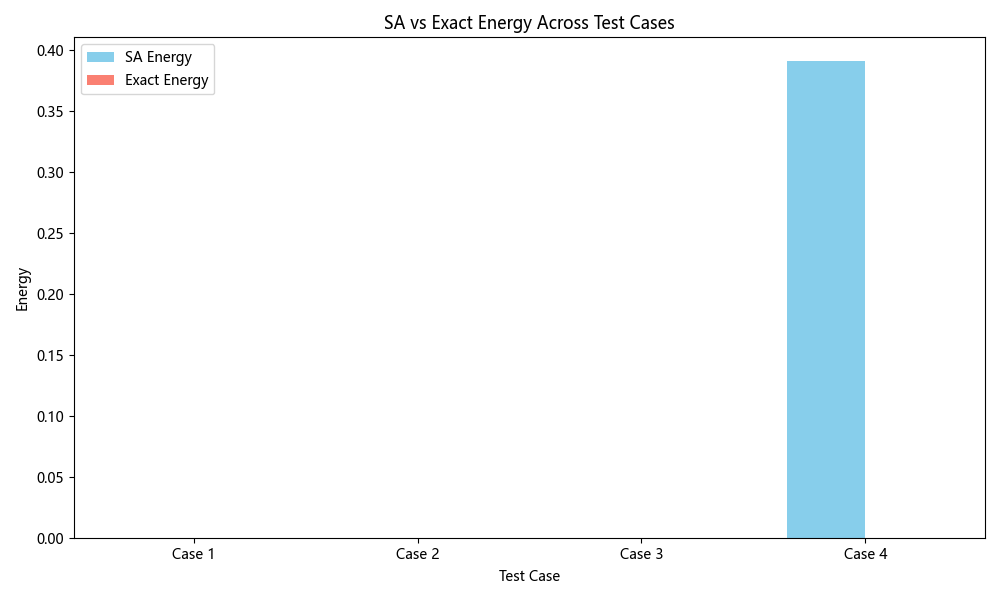
\includegraphics[width=\columnwidth]{energy_comparison.png} 
    \caption{整體能量比較:小規模精確解法、SA 皆 0;中大型精確解法 N/A,SA 有可行解}
\end{figure}

\FloatBarrier % 確保整體能量比較圖被放置

\subsection{整體時間比較}
以下為 SA 與精確解法的時間比較圖:

\begin{figure}[!htbp]
    \centering
   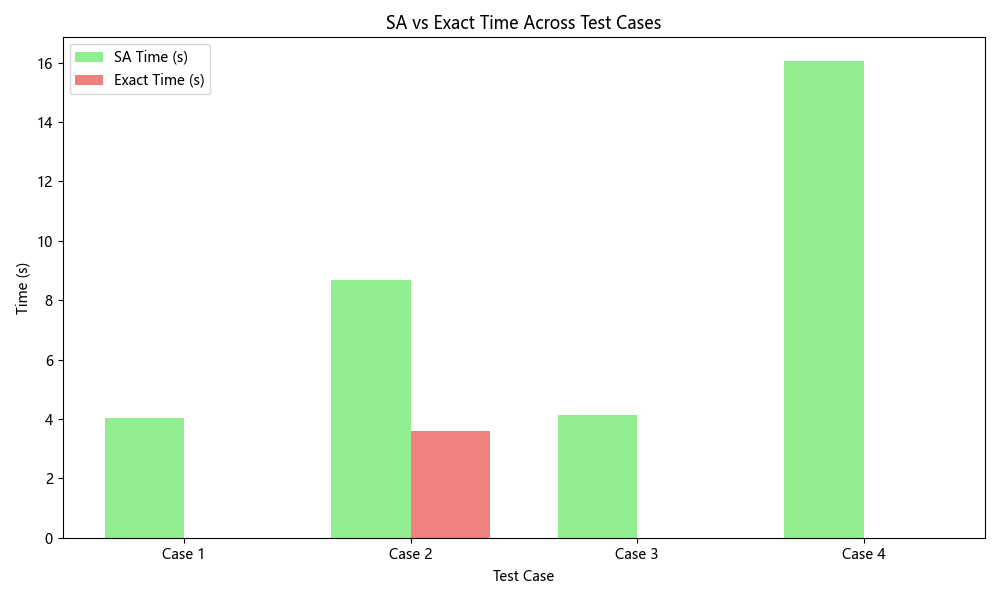
\includegraphics[width=\columnwidth]{time_comparison.png} 
    \caption{整體時間比較:小問題精確解法極快,SA 較久;中大型精確解法 N/A,SA 較久但有解}
\end{figure}

\FloatBarrier % 確保整體時間比較圖被放置

\subsection{結果表格彙整}
表 I 彙整四案例結果。

\begin{table}[!htbp]
\caption{四案例結果摘要}
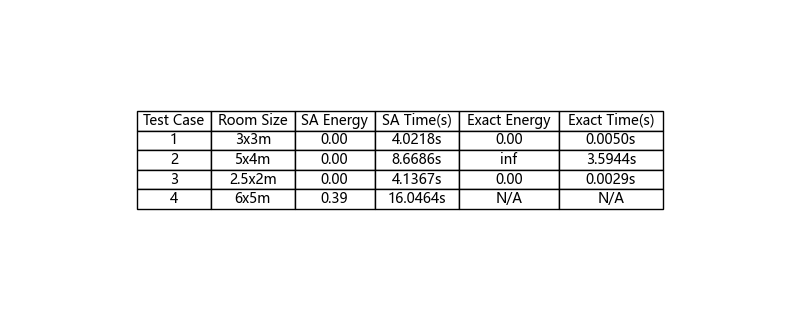
\includegraphics[width=\columnwidth]{results_comparison_table.png} 
\end{table}

\FloatBarrier % 確保表格被放置

\section{結論與展望}
本研究比較 SA 與精確解法在房間佈置優化問題下的表現。結果顯示:
\begin{itemize}
    \item 小規模問題:精確解法能在極短時間內求得能量 0 最優解,SA 亦可達 0 但較耗時。
    \item 中大型問題:精確解法無法求解(N/A),SA 雖耗時但仍可取得可行解。
\end{itemize}

未來可考慮混合策略(如先由精確解法求解局部,再以 SA 全域優化)或增加實務約束,使結果更貼近真實設計需求。

\FloatBarrier % 確保所有浮動物件在此之前被放置

\begin{thebibliography}{99}
\bibitem{b1} Kirkpatrick, S., Gelatt, C. D., \& Vecchi, M. P. (1983). Optimization by simulated annealing. \textit{Science}, 220(4598), 671–680. \url{https://doi.org/10.1126/science.220.4598.671}

\bibitem{b2} Woeginger, G. J. (2003). Exact algorithms for NP-hard problems: A survey. In Jünger, M., Reinelt, G., \& Rinaldi, G. (Eds.), \textit{Combinatorial Optimization—Eureka, You Shrink! (Lecture Notes in Computer Science, vol. 2570)}. Springer, Berlin, Heidelberg. \url{https://doi.org/10.1007/3-540-36478-1_17}
\end{thebibliography}

\end{document}
